\chapter{Analiza śladu pamięci}

W celu umożliwienia estymacji wymaganych zasobów sprzętowych w systemach opartych o protokół Thread, a w szczególności korzystających z implementacji OpenThread na platformie nRF52, dokonano badania, w którym analizowano stopień wykorzystania pamięci RAM oraz ROM (ang. \textit{Read-Only Memory}) po uruchomieniu stosu Thread oraz w zależności od wybranych funkcjonalności.

\section{Doświadczenie}

    \subsection{Założenia}

    Badanie przeprowadzono dla aplikacji dedykowanych platformie nRF52833 DK, stworzonych przy pomocy nRF Connect IDE. Do pomiarów wykorzystano narzędzia \textit{Memory Raport}, które jest częścią wspomnianego środowiska programistycznego. 
    
    W ramach analizy dokonywano modyfikacji stworzonego na potrzeby doświadczenia projektu, poprzez włączanie kolejnych funkcjonalności powiązanych ze stosem Thread. W kolejnym kroku porównywano zużycie RAM oraz ROM, dodatkowo wyszczególniając obszary pamięci, które zajmują najwięcej miejsca.

    Na Rysunku \ref{fig:memory-raport} przedstawiono zrzut ekranu prezentujący narzędzie Memory Raport.

    \begin{figure}[H]
        \centering
        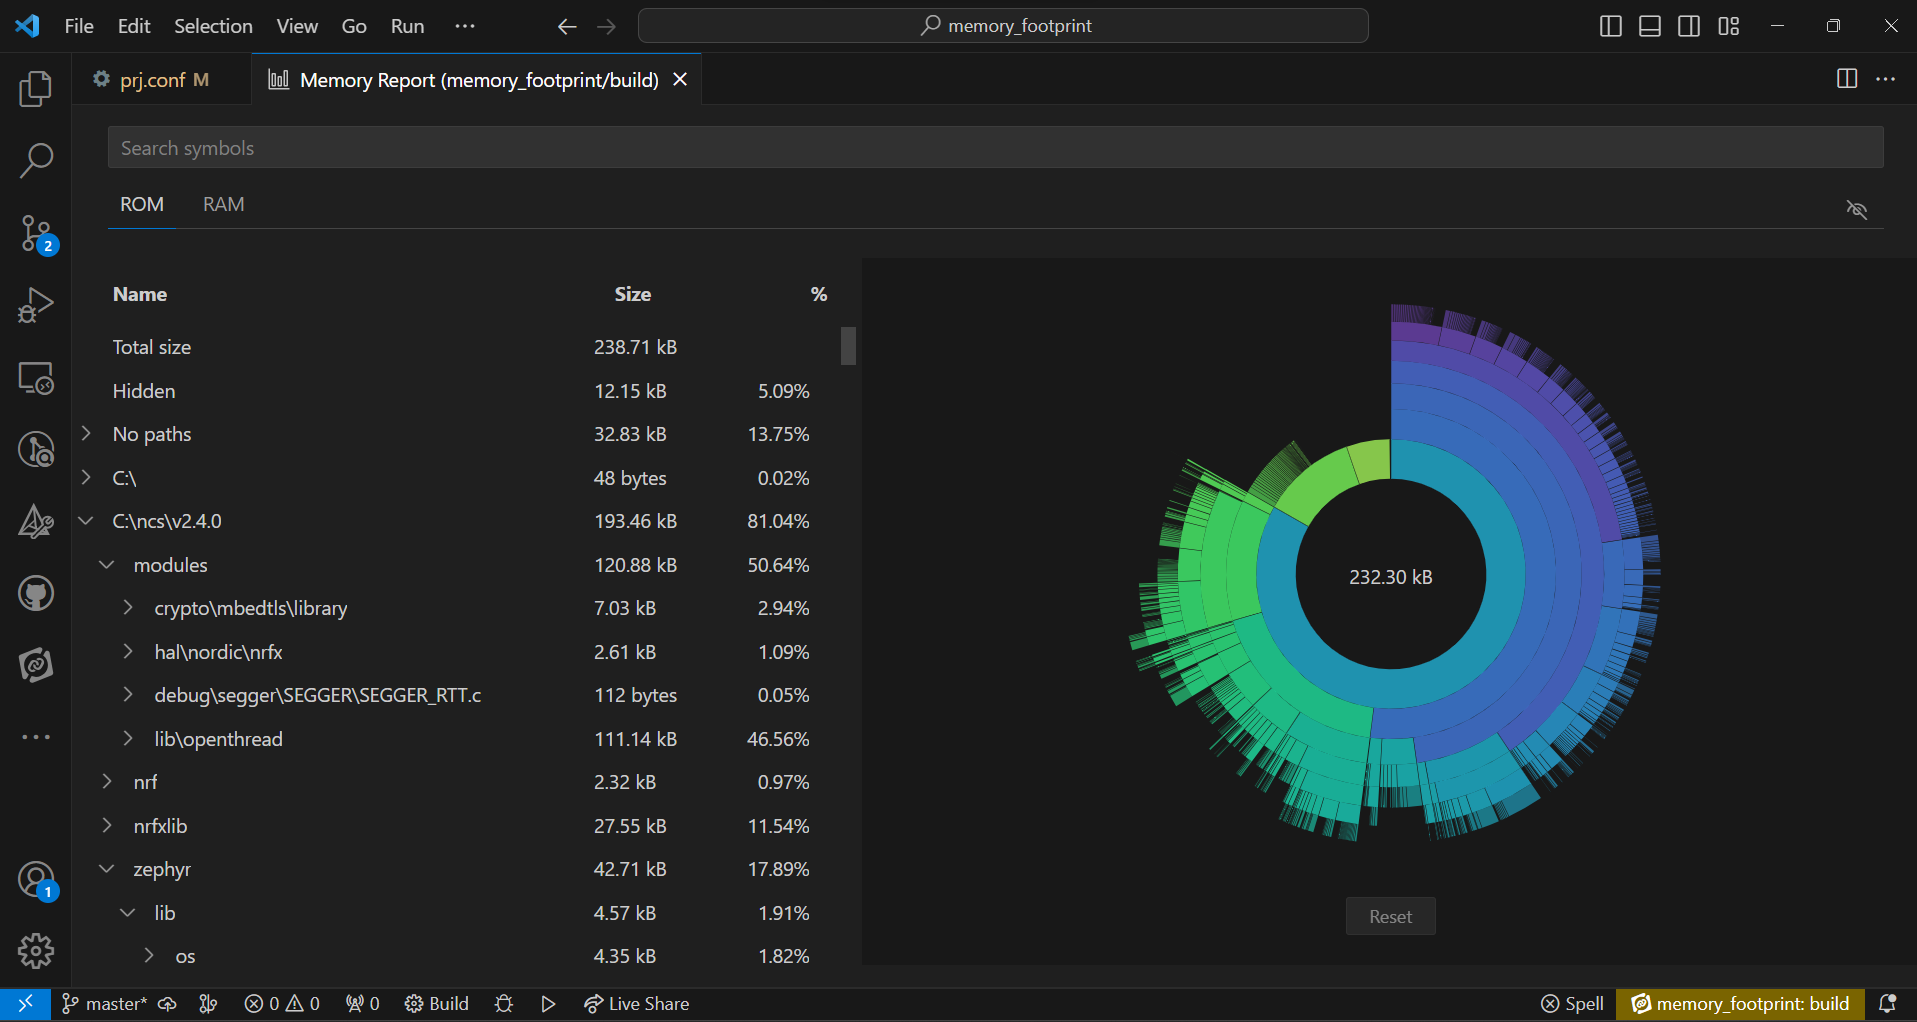
\includegraphics[width=0.8\linewidth]{graphics/memory-raport.png}
        \caption{Zrzut ekranu z narzędziem Memory Raport.}
        \label{fig:memory-raport}
    \end{figure}

    \subsection{Pomiar}
    \label{subsec:mem-footprint-measure}

        \subsubsection{Projekt bez dodatkowych konfiguracji}
        
        W celu ustalenia punktu odniesienia zbudowano projekt bez uwzględniania jakichkolwiek dodatkowych opcji konfiguracji.
        Uzyskane zużycie pamięci zestawiono na pozycji \textit{1} w Tabeli \ref{tab:memory-measures}.
        
        Zauważono, że większość wykorzystanego ROM związana jest z uruchomieniem systemu operacyjnego Zephyr i jest skojarzona z uwzględnieniem sterowników sprzętowych oraz warstwy HAL (ang. \textit{Hardware Abstraction Layer}). W przypadku pamięci RAM, większość zasobów została poświęcona na stos przerwań oraz na inicjalizację jądra systemu operacyjnego.

        \subsection{Projekt z opcją networking}

        Do inicjalizacji stosu Thread, niezbędnym jest skonfigurowanie warstwy sieciowej IP oraz funkcjonalności z nią związanych. W tym celu wzbogacono projekt o parametr konfiguracyjny \textit{CONFIG\_NETWORKING}, który uwzględnia w aplikacji warstwę łącza danych oraz warstwę sieciową z protokołem IP.
        Uzyskane zużycie pamięci zestawiono na pozycji \textit{2} w Tabeli \ref{tab:memory-measures}.

        \subsection{Projekt z włączonym stosem Thread v1.3}

        Po włączeniu warstwy sieciowej projekt jest przygotowany na wystartowanie protokołu Thread w implementacji OpenThread. Dodano do pliku konfiguracyjnego opcję \textit{CONFIG\_NET\_L2\_OPENTHREAD}, która konfiguruje LR-WPAN oraz uwzględnia funkcjonalności niezbędne do uruchomienia stosu Thread. Uzyskane zużycie pamięci zestawiono na pozycji \textit{3} w Tabeli \ref{tab:memory-measures}.

        Uwzględnienie stosu Thread spowodowało ponad czterokrotny wzrost zużycia ROM oraz niemalże czterokrotnie większe wykorzystanie RAM. 
        
        Najwięcej zasobów pamięci nieulotnej jest pochłanianych przez bibliotekę OpenThread, uwzględnioną przez nRF Connect SDK. Rozmiar sekcji pamięci przeznaczonej dla biblioteki OpenThread wynosi 94,01 kB. Stos Thread wymaga odbioru ramek IEEE 802.15.4. Obszar dedykowany dla sterowników do konfiguracji LR-WPAN zajął 27,31 kB.

        Wysokie zużycie RAM jest spowodowane koniecznością alokacji sekcji pamięci dla kontekstu sieci Thread, zastosowań kryptograficznych Mbed TLS oraz obsługi radia LR-WPAN. Sekcja przeznaczona na kontekst \textit{ot::gInstanceRaw} zajmuje 27,44 kB, natomiast obszar wykorzystywany przez Mbed TLS zużywa 12,92 kB.

    \subsection{Projekt z włączonym stosem Thread w wersji 1.1 oraz 1.2}

    W celu porównania zużycia zasobów sprzętowych między kolejnymi wersjami Thread dokonano pomiaru wykorzystania RAM oraz ROM również dla wersji 1.1 oraz 1.2., dodając do pliku konfiguracyjnego parametr \textit{CONFIG\_OPENTHREAD\_THREAD\_VERSION\_1\_1} lub \\ \textit{CONFIG\_OPENTHREAD\_THREAD\_VERSION\_1\_2}. Uzyskane zużycie pamięci zestawiono na pozycji \textit{4} oraz \textit{5} w Tabeli \ref{tab:memory-measures}.

    Niewielka różnica w wielkości wykorzystanych zasobów RAM oraz ROM między wersją 1.1 a 1.2, oraz 1.3 wynika z konieczności uwzględnienia dodatkowych mechanizmów i funkcjonalności w sieci Thread \cite{nrf-thread-version-options}, takich jak \textit{Coordinated Sampled Listening}, \textit{Link Metrics Probing}, \textit{Multicast across Thread networks}, \textit{Thread Domain unicast addressing}, \textit{Enhanced Frame Pending, Enhanced Keep Alive}.

    Ostatecznie, dla kolejnych rozważań, przywrócono konfigurację stosu Thread do wersji 1.3.

    \subsection{Projekt z włączonym stosem Thread dla różnych typów urządzeń}

    Domyślnym typem urządzenia dla skonfigurowanej aplikacji z włączonym stosem Thread jest FTD. W celu zbadania zużycia zasobów pamięci dla projektu, w którym urządzenie działa jako MTD, nadpisano konfigurację, dodając do pliku konfiguracyjnego parametr \textit{CONFIG\_OPENTHREAD\_MTD}. Co więcej, zmieniono konfigurację projektu, dodając opcję \textit{CONFIG\_OPENTHREAD\_MTD\_SED}, aby zbadać zmianę użytych zasobów dla urządzenia SED. Uzyskane zużycie pamięci zestawiono na pozycji \textit{6} oraz \textit{7} w Tabeli \ref{tab:memory-measures}.

    Można zauważyć, że przełączenie konfiguracji na MTD obniża zużycie zarówno ROM jak i RAM. Urządzenia typu MTD posiadają zredukowany zestaw funkcjonalności w sieci Thread, jak np. nie są w stanie przekazywać pakietów do innych węzłów. Potwierdza to zmniejszona, w stosunku do przypadku 5, sekcja pamięci nieulotnej, dedykowana dla biblioteki OpenThread, której rozmiar wynosi 64,07 kB, jak również redukcja rozmiaru kontekstu sieci \textit{ot::gInstanceRaw} do wielkości 18,48 kB.

    Na skutek dodania funkcjonalności SED, nie zmierzono zmian w zużyciu zasobów pamięci.

    Na koniec przywrócono w projekcie rolę FTD.

    \subsection{Projekt z włączonym stosem Thread oraz skonfigurowanym mechanizmem Commissioning}
    Projekt ze skonfigurowanym stosem Thread w wersji 1.3 wzbogacono o funkcjonalności związane z mechanizmem Commissioning. Do pliku konfiguracyjnego dodano opcję \\\textit{CONFIG\_OPENTHREAD\_COMMISSIONER}, aby ustalić rolę Commissioner urządzenia, a następnie \\\textit{CONFIG\_OPENTHREAD\_JOINER} w celu konfiguracji roli Joiner. Uzyskane wartości zużytej pamięci zestawiono na pozycji \textit{8} oraz \textit{9} w Tabeli \ref{tab:memory-measures}.
    
    Po dokonaniu pomiaru wyłączono mechanizm Commissioning.

    \subsection{Projekt z włączonym stosem Thread oraz ze skonfigurowaną konsolą OpenThread CLI}

    Aby umożliwić konfigurację urządzeń w sieci Thread poprzez użycie OpenThread CLI, niezbędne jest skonfigurowanie konsoli Shell. Utworzono nowy projekt, w którym skonfigurowano tylko konsolę. Zmierzono zużycie zasobów i zestawiono na pozycji \textit{10} w Tabeli \ref{tab:memory-measures}. Kolejno powrócono do projektu ze stosem Thread v1.3 dla urządzenia FTD, a następnie włączono funkcjonalności konsoli Shell oraz dodatkowo skonfigurowano OpenThread CLI. Wykorzystany RAM oraz ROM po uwzględnieniu w projekcie OpenThread CLI zestawiono na pozycji \textit{11} w Tabeli \ref{tab:memory-measures}.
        
    \begin{table}[H]
        \centering
        \caption{Zużycie zasobów pamięci dla kolejno omwaianych przypadków.}
        \begin{tabular}{|l|l|l|l|}
            \hline
            \rowcolor{gray!20}
            \multicolumn{1}{|c|}{l.p.} & \multicolumn{1}{c|}{ROM [kB]} & \multicolumn{1}{c|}{RAM [kB]} & \multicolumn{1}{c|}{Opis} \\
            \hline
            1 & 19,11 & 5,78 & Brak dodatkowych konfiguracji\\
            \hline
            2 & 51,39 & 18,81 & Konfiguracja L2 oraz L3 IP\\
            \hline
            3 & 217,18 & 72,76 & Stos Thread v1.3, FTD\\
            \hline
            4 & 217,18 & 72,76 & Stos Thread v1.2, FTD\\
            \hline
            5 & 211,20 & 71,46 & Stos Thread v1.1, FTD\\
            \hline
            6 & 177,44 & 63,80 & Stosu Thread v1.3, MTD\\
            \hline
            7 & 177,44 & 63,80 & Stos Thread v1.3, MTD, SED\\
            \hline
            8 & 251,26 & 76,84 & Stos Thread v1.3, FTD, Commissioner\\
            \hline
            9 & 245,96 & 76,52 & Stos Thread v1.3, FTD, Joiner\\
            \hline
            10 & 42,99 & 11,44 & Konfiguracja konsoli Shell\\
            \hline
            11 & 304,32 & 87,43 & Stos Thread v1.3, FTD Openthread CLI \\
            \hline
        \end{tabular}
        \label{tab:memory-measures}
    \end{table}

    W Tabeli \ref{tab:component-memory-usage} przedstawiono oszacowane wartości zużytych RAM oraz ROM dla analizowanych funkcjonalności, które zostały obliczone na podstawie różnic między wartościami zasobów umieszczonych w Tabeli \ref{tab:memory-measures}.

    \begin{table}[H]
        \centering
        \caption{Zużycie zasobów pamięci przez wybrane komponenty.}
        \begin{tabular}{|l|l|l|l|}
            \hline
            \rowcolor{gray!20}
            \multicolumn{1}{|c|}{Funkcjonalność} & \multicolumn{1}{c|}{ROM [kB]} & \multicolumn{1}{c|}{RAM [kB]} & \multicolumn{1}{c|}{Wymagana funkcjonalność} \\
            \hline
            Inicjalizacja Zephyr & 19,11 & 5,78 & brak\\
            \hline
            Networking & 32,28 & 13,03 & Inicjalizacja Zephyr\\
            \hline
            Konsola Shell & 23,88 & 5,66 & Inicjalizacja Zephyr\\
            \hline
            Stos Thread v1.3 dla FTD & 165,79 & 53,95 & Networking\\
            \hline
            Stos Thread v1.3 dla MTD & 126,05 & 44,99 & Networking\\
            \hline
            Rola Commissioner dla FTD & 40,06 & 4,08 & Stos Thread v1.3 dla FTD\\
            \hline
            Rola Joiner dla FTD & 28,16 & 3,76 & Stos Thread v1.3 dla FTD\\
            \hline
            OpenThread CLI dla FTD & 44,15 & 12,19 & Stos Thread v1.3 dla FTD, Konsola Shell\\
            \hline
        \end{tabular}
        \label{tab:component-memory-usage}
    \end{table}

\section{Wnioski}

Przeprowadziwszy analizę zużycia zasobów pamięci dla funkcjonalności protokołu Thread, na platformie nRF52833 w implementacji Openthread, wysunięto następujące wnioski.

Uruchomienie OpenThread wymaga dołączenia biblioteki, która w stosunku do innych wykorzystanych sekcji ROM, wymaga dużej liczby dostępnej pamięci nieulotnej. Nie jest możliwym na podstawie przeprowadzonej obserwacji, aby stwierdzić, czy uwzględnienie całej biblioteki załączonej do pamięci nieulotnej, jest niezbędne do poprawnego działania stosu Thread. Jeżeli w użytej bibliotece są zawarte fakultatywne funkcjonalności, istniałaby możliwość na optymalizację zużycia zasobów, poprzez selektywny dobór tylko tych funkcjonalności, który są konieczne do zapewnienia zgodnego ze standardem \cite{thread-1.3.0} działania sieci Thread.

Największe zużycie RAM spowodowane jest potrzebą zaalokowania w pamięci ulotnej obszaru dla kontekstu sieci Thread oraz zmiennych wykorzystywanych w zastosowaniach kryptograficznych. Domyślną biblioteką algorytmów szyfrowania, która została uwzględniona przy uruchomieniu OpenThread, jest Mbed TLS. W celu ewentualnej optymalizacji zużytych zasobów pamięci, sugerowane jest porównanie wykorzystanej implementacji z innymi, otwartymi, dostępnymi bibliotekami TLS (ang. \textit{Transport Layer Security}), takimi jak np. \textit{OpenSSL}, \textit{libsodium}, \textit{Crypto++} \cite{mbed-tls-alt}. 

Rola MTD wymaga mniejszych zasobów niż FTD. Urządzenia końcowe pracujące jako MED, pełniące rolę czujników i regulatorów, są w stanie posiadać mniejsze zasoby pamięci, niezbędne do poprawnego działania. Z kolei do uruchomienia urządzeń pracujących jako Rutery, konieczne jest uwzględnienie większego zaplecza pamięci. Ponadto włączenie roli Commissioner zużywa więcej RAM oraz ROM, aniżeli uruchomienie roli Joiner. Urządzeniem Commissioner może być tylko Ruter, co wprowadza dodatkowe wymagania odnośnie dostępnej pamięci.

W przypadku potrzeby wykorzystywania konsoli OpenThread CLI, zalecane jest, aby wykorzystać urządzenie o pamięci RAM oraz ROM większej o liczbę przedstawioną w Tabeli \ref{tab:component-memory-usage}. Włączenie konsoli OpenThread nie jest niezbędne, natomiast może być pomocna w przypadku chęci dynamicznej konfiguracji sieci Thread w trakcie działania aplikacji, szczególnie na takich urządzeniach jak Rutery czy Rutery Brzegowe.




